% Figures and legends.

\begin{figure}[p]
  \centering
  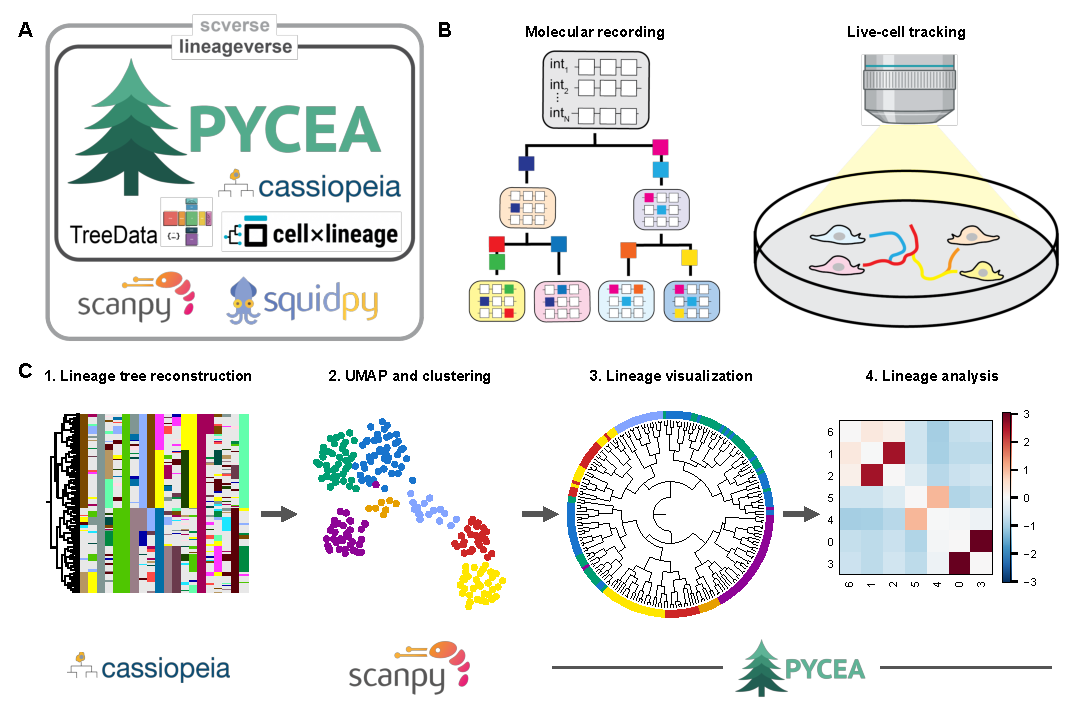
\includegraphics[width=\textwidth]{figure1.pdf}
  \caption{\textbf{Pycea integrates lineage tracing analysis into the scverse ecosystem.}
  \textbf{(A)} Pycea and TreeData within the scverse and lineageverse ecosystems.
  \textbf{(B)} Supported lineage tracing data: molecular recording (left) and live-cell tracking (right).
  \textbf{(C)} Example workflow on single-cell lineage tracing data: (1)~lineage tree reconstruction with Cassiopeia, (2)~UMAP and Leiden clustering with Scanpy, (3)~polar tree with leaves annotated by cluster, and (4)~ancestral linkage between clusters with Pycea.}
  \label{fig:overview}
\end{figure}

\begin{figure}[p]
  \centering
  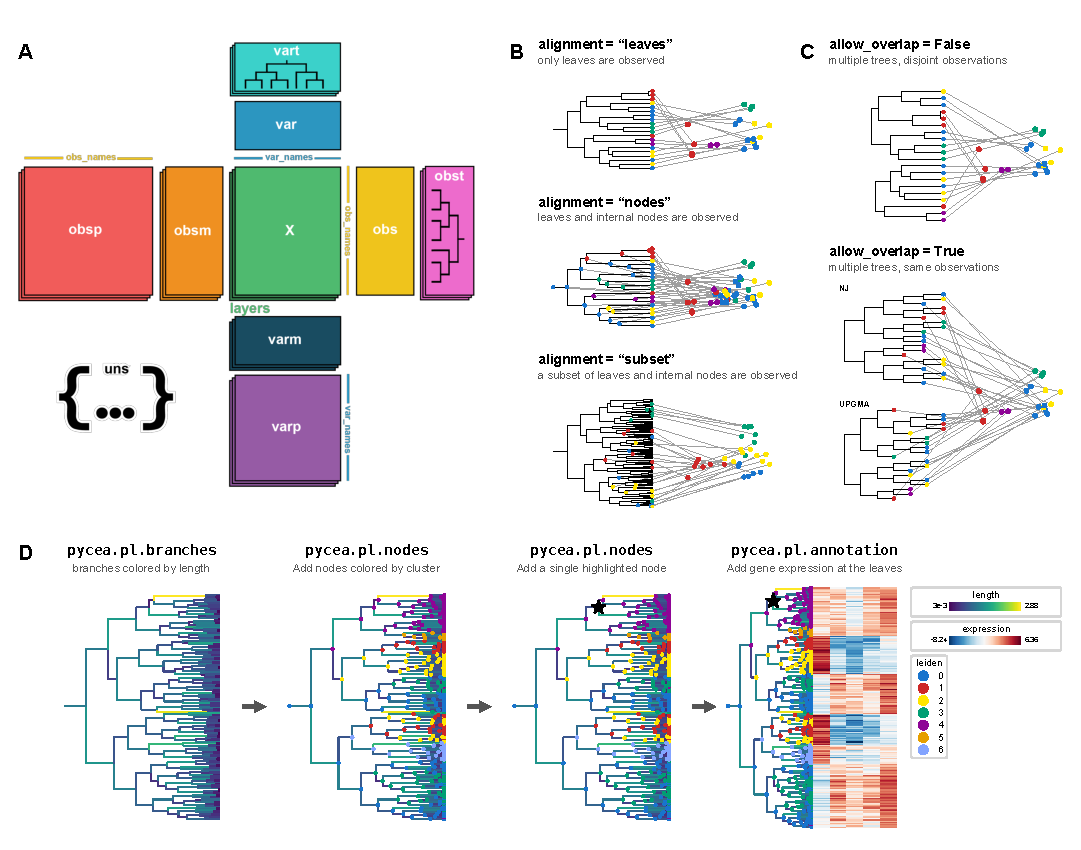
\includegraphics[width=\textwidth]{figure2.pdf}
  \caption{\textbf{The TreeData object stores one or more trees aligned to observations.}
  \textbf{(A)} TreeData extends AnnData with \code{obst} and \code{vart} fields, which store trees aligned to observations and variables.
  \textbf{(B)} Alignment modes. Gray lines connect tree nodes to their observations in the UMAP. With \code{"leaves"}, only leaves are observations; with \code{"nodes"}, leaves and internal nodes are; with \code{"subset"}, only some nodes are.
  \textbf{(C)} Multiple trees per object: trees with disjoint observations (\code{allow_overlap=False}, top) or multiple trees for the same observations (\code{allow_overlap=True}, bottom; neighbor-joining (NJ) and UPGMA).
  \textbf{(D)} A tree plot built up with successive Pycea calls: \code{pycea.pl.branches} (branches colored by length), \code{pycea.pl.nodes} (leaves and internal nodes colored by cluster; then a single node highlighted), and \code{pycea.pl.annotation} (expression of five genes at the leaves).}
  \label{fig:treedata}
\end{figure}

\begin{figure}[p]
  \centering
  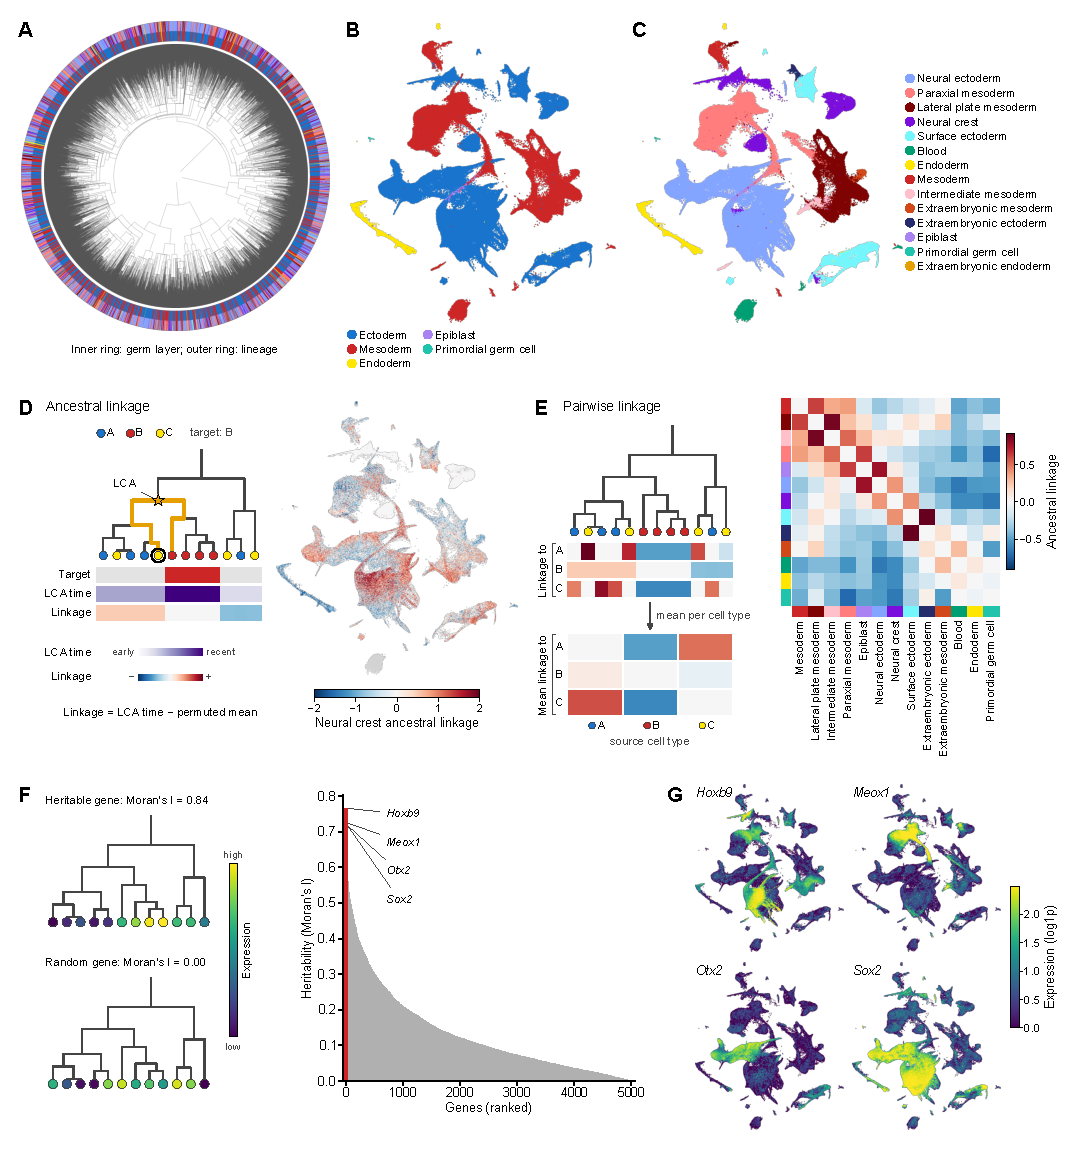
\includegraphics[width=\textwidth]{figure3.pdf}
  \caption{\textbf{Fate restriction in a mouse embryo.}
  \textbf{(A)} Lineage trees of an E9.5 embryo (262,534 cells) with leaves annotated by germ layer (inner ring) and lineage (outer ring).
  \textbf{(B, C)} UMAP of cells colored by germ layer (B) and broad lineage annotation (C).
  \textbf{(D)} Ancestral linkage of a cell to a target set is the time of its most recent common ancestor (LCA) with the nearest target cell, normalized to chance (left). UMAP colored by neural crest ancestral linkage (right); gray cells are not in a lineage tree.
  \textbf{(E)} Pairwise linkage: the mean linkage of each cell type to a target cell type forms one row, repeated with every cell type as the target (left), giving the symmetrized linkage between all lineages (right; colors as in C).
  \textbf{(F)} Heritable genes have expression that is autocorrelated across the lineage tree, measured by Moran's I (left), shown ranked for the 5,000 highly variable genes (right).
  \textbf{(G)} UMAPs colored by expression of the four most heritable genes.}
  \label{fig:embryo}
\end{figure}

\begin{figure}[p]
  \centering
  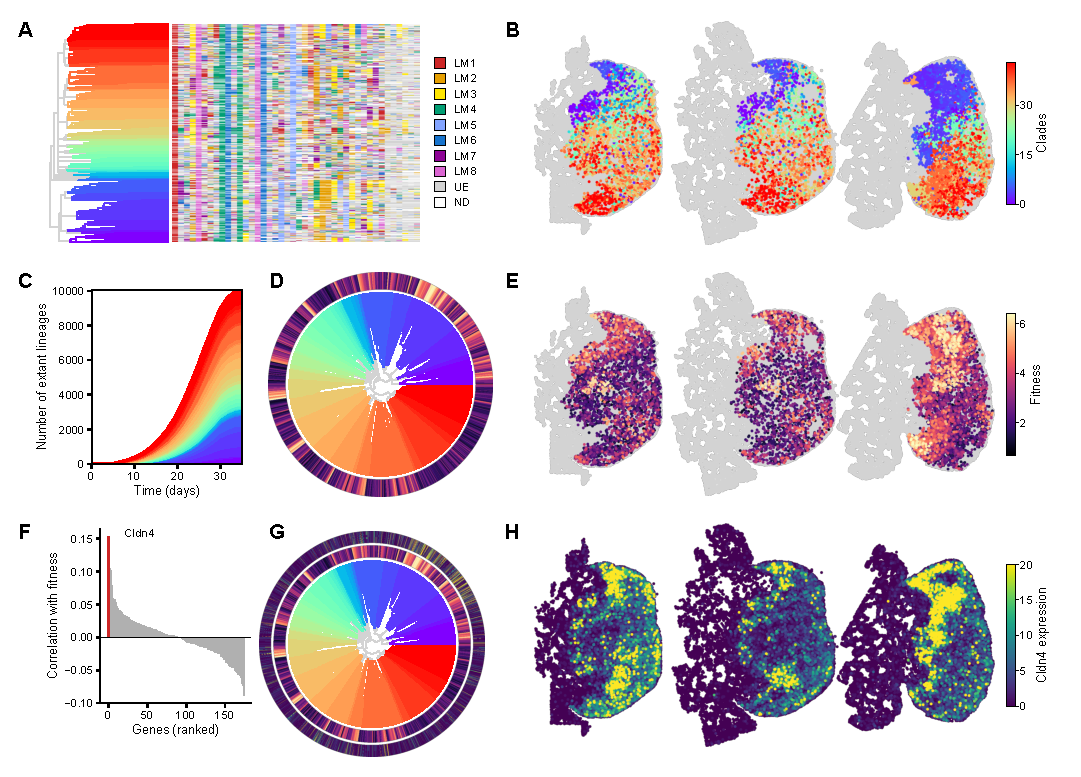
\includegraphics[width=\textwidth]{figure4.pdf}
  \caption{\textbf{Growth dynamics of a 4T1 tumor.}
  \textbf{(A)} Lineage tree and character matrix, with branches colored by clade (cells sharing an ancestor at day 5); colors indicate lineage marks (LMs), gray unedited (UE), and white no detection (ND).
  \textbf{(B)} Spatial distribution of clades across three tumor sections; gray cells are not in the lineage tree.
  \textbf{(C)} Number of extant lineages in each clade over time (\code{pycea.pl.n_extant}).
  \textbf{(D)} Polar tree with the estimated fitness (\code{pycea.tl.fitness}) of each cell in the outer ring.
  \textbf{(E)} Spatial distribution of fitness.
  \textbf{(F)} Correlation of gene expression with fitness; \textit{Cldn4} is highlighted.
  \textbf{(G)} Polar tree with rings for fitness and \textit{Cldn4} expression.
  \textbf{(H)} Spatial distribution of \textit{Cldn4} expression.}
  \label{fig:growth}
\end{figure}

% ---- Supplementary information: figures are numbered S1, S2, ... ----
\setcounter{figure}{0}
\renewcommand{\thefigure}{S\arabic{figure}}
\begin{figure}[p]
  \centering
  {\large\textbf{Supplementary Information}}\par\medskip
  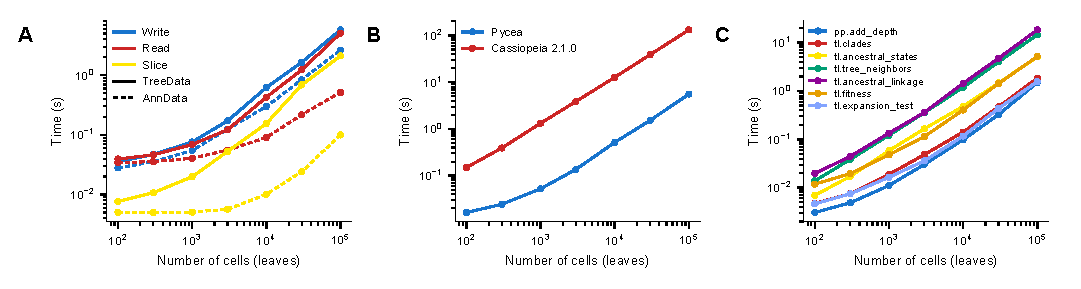
\includegraphics[width=\textwidth]{figureS1.pdf}
  \caption{\textbf{Benchmarks.}
  \textbf{(A)} Time to write, read and slice (a random 10\% of cells) TreeData and AnnData objects with a simulated lineage tree and simulated expression of 20,000 genes (sparse counts), by number of cells.
  \textbf{(B)} Time to plot a tree with Pycea and with Cassiopeia 2.1.0 (plotting deprecated in version 3.0.0), by number of cells.
  \textbf{(C)} Run time of key Pycea functions, by number of cells. Median of three runs, on a single node.}
  \label{fig:benchmarks}
\end{figure}
